\chapter{Related Work}
\label{ch:related-work}

Multiple attempts have been undertaken to use the Semantic Web as it was envisioned by Berners-Lee et al.\@~\cite{berners2001semantic}
as a research dataset.
Thereby, the data that was previously hidden in the unstructured HTML files is used as an additional feature generation method
for ontology matching and catalog integration~\cite{meusel2015exploiting, sabou2008exploring}.
Today, the field of ontology matching is an active research area with contributions utilizing external
corpora~\cite{giunchiglia2005semantic, park2007ontology, aanen2012schema} like WordNet~\cite{miller1995wordnet},
embeddings~\cite{zhang2014ontology, portisch2018alod2vec}, and other machine learning approaches~\cite{doan2004ontology}.
Some methods focus explicitly on the task of product taxonomy matching~\cite{vandic2012faceted, park2007ontology, aanen2012schema}.

The first Section in this Chapter introduces contributions that use the Semantic Web as the underlying dataset for their research.
They use Semantic Web data for ontology matching or with a focus on products from e-commerce platforms.
We introduce taxonomy matching algorithms in the second Section and focus on product taxonomy matching in the
third Section.
We conclude this Chapter with a categorization of the presented approaches.

\section{Semantic Web}
\label{sec:rw-semantic-web}

Sabou et al.\@~\cite{sabou2008exploring} propose the use of information encoded in the Semantic Web as background
knowledge for ontology matching tasks.
They name numerous ontology matching approaches that rely on an external ontology as background knowledge,
e.g., the work of Aleksovski et al.\@~\cite{aleksovski2006matching}.
In their article Sabou et al.\@ validate the hypothesis that a set of ontologies extracted from the
Semantic Web covers a larger universe and contains more knowledge than any single ontology which is currently available or
can be manually crafted for a single experiment.
Instead of using a single ontology as background knowledge, they use multiple, automatically selected ontologies.
Their goal is to use the background ontology with the best coverage of the given domain.
Sabou et al.\@ found that using the Semantic Web leads to results comparable to existing methods, although
the semantic relations on the web are often erroneous, especially with regard to subsumption relationships.
Overall, they conclude that ontologies extracted from the Semantic Web can serve as background knowledge in order
to improve existing mapping methods.

In 2014 Meusel et al.\@~\cite{meusel2014webdatacommons} laid the foundation for many experiments using data from the
Semantic Web by publishing the WDC Microdata, RDFa and Microformat Dataset Series.
Based on the extracts published by the Common Crawl project, they produced
a set of over 30 billion RDF quads.
The layout of an RDF quad with additional examples is explained in Section~\ref{sec:retrieve-product-semantic-web}.
In addition to the raw extraction results, class-specific subsets are published
annually\footnote{\url{http://webdatacommons.org/structureddata/2019-12/stats/schema_org_subsets.html}. Accessed: 01.05.2020}.
The latest results based on the 2019 Common Crawl contains more than 900 million quads from more than 218,000 hosts
for product-related classes.
Multiple authors reuse those results for their own research, e.g.,~\cite{meusel2015exploiting, petrovski2016wdc, zhang2019product}.

In a follow-up paper, Meusel et al.\@~\cite{meusel2015exploiting} reused those results to improve product categorization
in e-commerce catalog integration tasks.
First, they extracted statistics about properties that occur in the Product/Offer annotations and found that about 86 percent
of the Pay-Level Domains (PLD) contain a name, 66 percent an image and/or a description, but only 2 percent of the PLDs annotate their products
with a category or breadcrumb.
The categories and breadcrumbs form the taxonomy of an individual PLD and contain the class of the given product.
Those classes are relevant for the remainder of their paper and also, later, for our work.
The goal of Meusel et al.\@ is to use the annotated properties, especially the class-property, to classify products into the
GPC's taxonomy.
From the annotation data a gold standard was created and used to evaluate product classification methods.
During the process, Meusel et al.\@ encoded their product information as vectors with a Bag-of-Words (BoW) and a
tf-idf approach and applied multiple classifiers, namely Naive Bayes, Decision Trees, and k-Nearest-Neighbors.
They show that it is possible to predict the product class with an 80 percent accuracy in a supervised approach.

Zhang and Paramita~\cite{zhang2019product} build on the dataset and ideas of Meusel et al.\@~\cite{meusel2015exploiting},
but use new classification methods based on deep-learning models and achieve a significant improvement with regard to the
F1-score.
Instead of encoding the product data as vectors with BoW or tf-idf, they use a GloVe word-embedding model~\cite{pennington2014glove}
that was pre-trained on the Common Crawl corpus.
In their work, they also considered a word2vec word-embedding model~\cite{mikolov2013distributed} pre-trained on
a Google News\footnote{\url{https://code.google.com/archive/p/word2vec/}. Accessed: 01.05.2020} corpus, but
expected a higher coverage with the Common Crawl model since the data is also extracted from the same corpus.
Zhang and Paramita state that in most classification papers, the name property is combined with additional metadata
as an input for the classifier.
Contrary to this approach, they also use the description and the class-label as individual inputs and try
combinations of those three features.
Here, the class-labels are encoded as a weighted sum of the word-embeddings that make up the class-label.
In addition, Zhang and Paramita experimented with different cleaning and normalization steps on the class-label
and discovered that they were counterproductive for the product classification task since relevant
contextual information was discarded.
Overall, they demonstrate that word-embeddings on the class-labels of products are a useful input for classification tasks.

Another use of product data from the Semantic Web is given by Primpeli et al.\@~\cite{primpeli2019wdc, petrovski2016wdc}.
They use the class-specific product dataset published by the WDC project to create a large training set and gold standard
for product matching on realistic, web-scale data.
Afterwards, they apply existing approaches for entity resolution on this dataset and try to replicate the results from
other contributions that were tested on smaller datasets.
In order to create the training dataset Primpeli et al.\@ pick schema.org properties that point to product identifiers, clean
them, and perform a similarity search on the identifiers to find products that have the same underlying identity.
They manually validate a subset of 2,200 products of those matches and, in the end, provide three datasets:
the complete training dataset, a subset from English domains, and a manually verified gold standard.
The complete training dataset consists of 26 million offers and the English subset of 16 million offers.
Their baseline experiments on the newly created datasets achieve an F1-score of 0.9 for entity resolution and, therefore,
prove the utility of this training data from more than 79,000 e-commerce platforms.

\section{Ontology/Taxonomy Matching}
\label{sec:rc-ontology-matching}

We will focus on general ontology matching with a special focus on taxonomy matching in this Section.
In the first part textbooks and surveys are introduced, which may serve as a reference for a more profound, general
introduction into the  topic of ontology matching.
Next, catalog integration papers are introduced.
Their relevance for this Thesis stems from the fact that properties of ontologies are used for a classification task.
Towards the end of this Section, we will take a closer look at taxonomy matching approaches.

\subsection{Overviews}

The  Ontology Matching textbook by Euzenat and Shvaiko~\cite{euzenat2007ontology} introduces ontology
matching and includes a multitude of applications and models.
If one is interested in the topic of ontology matching beyond the task of taxonomy matching, this should serve as a
good starting point.

Euzenat and Shvaiko also provide a classification of ontology matching approaches shown in Figure~\ref{fig:ontology-matching-classification}.
\begin{figure}[!htbp]
    \centering
    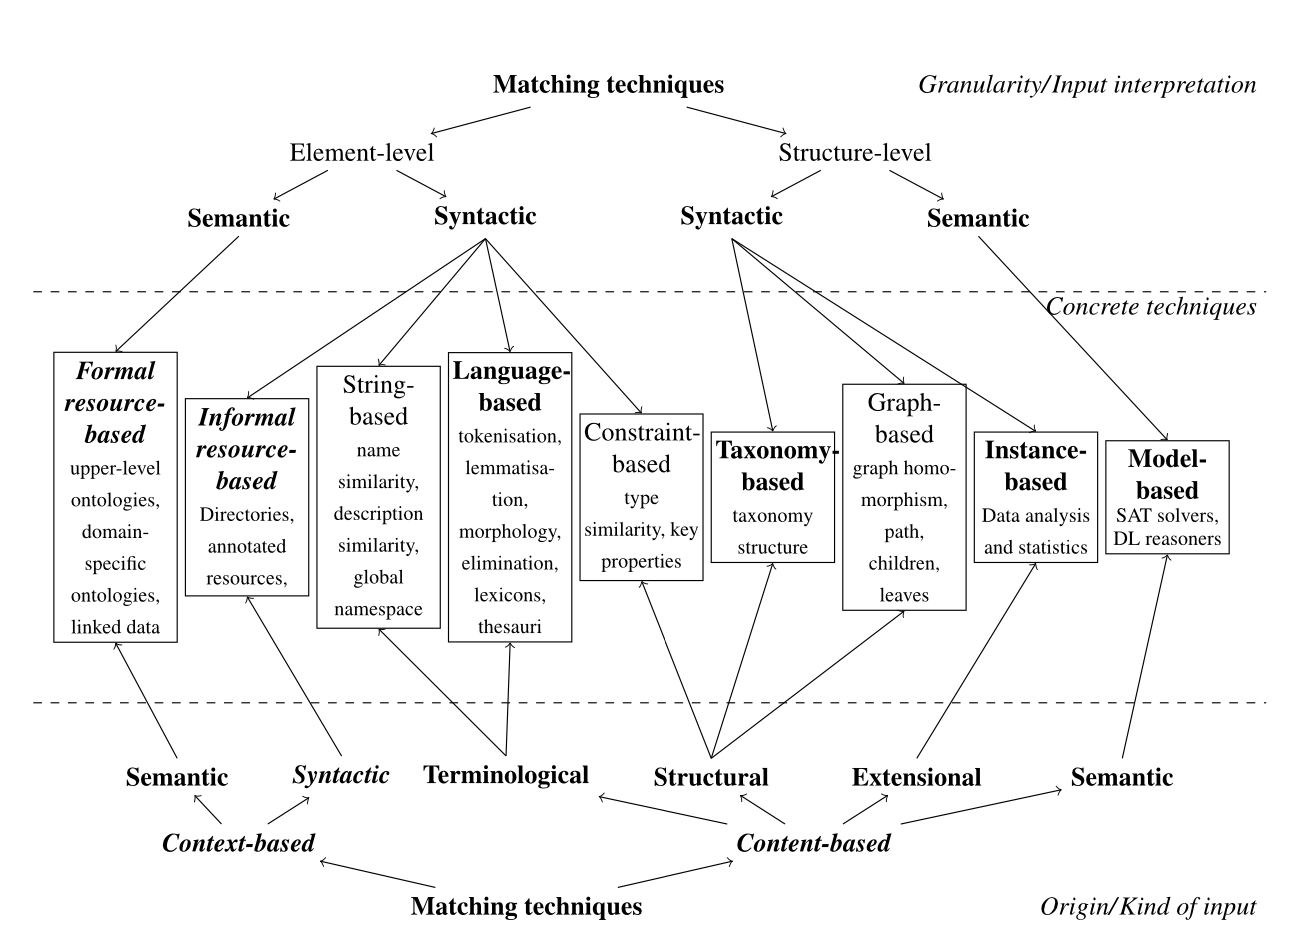
\includegraphics[width=13cm]{images/ontology-matching-classification.png}
    \caption[Ontology Matching Classification]{Ontology Matching Classification~\cite{euzenat2007ontology}}
    \label{fig:ontology-matching-classification}
\end{figure}
They define two high-level approaches to separate the specific techniques.
At the top, we see the classification based on granularity and at the bottom the classification based on origin.
Note that the techniques placed in the middle are shared among them.
The classification based on granularity distinguishes between element-level matchers and structure-level matchers.
The former compares only two entities at a time together with their properties, while the latter
takes the whole ontology into account to predict the most probable alignment.
The origin-based classification distinguishes based on the source of information that is used in
the classifier.
Content-based methods focus only on the content of the given ontologies, while context-based matchers allow external
knowledge resources, e.g., external ontologies from the Semantic Web as in~\cite{sabou2008exploring}.

Angerman and Ramzan published a textbook focusing exclusively on taxonomy matching approaches~\cite{angermann2017taxonomy}.
First, they introduce the problem of taxonomy matching by contrasting it to general ontology matching and motivate the work by introducing
use cases for taxonomy matching in the real world.
They also reuse ideas from Euzenat and Shvaiko~\cite{euzenat2007ontology}, especially the categorization based on Granularity
and the different sources of heterogeneity in taxonomies, namely terminological, conceptual, syntactical, and semiotic.
They define those concepts as follows~\cite[p.18]{angermann2017taxonomy}:
\begin{itemize}
    \item "\emph{Terminological Heterogeneity} appears when the concepts of two taxonomies are expressed using different languages [, e.g., English and German].
    \item \emph{Conceptual Heterogeneity} arises if two taxonomies use different relationships to describe an identical domain. [\ldots].
    \item \emph{Syntactical Heterogeneity} occurs when for the storage of the taxonomies different data languages/models are used. [\ldots].
    \item \emph{Semiotic Heterogeneity} emerges when persons misinterpret concepts, respectively the relationships inside the taxonomies along with the used labels for concepts. [\ldots]."
\end{itemize}
In the second part of their book, they survey state-of-the-art taxonomy matching algorithms from recent
OAEI campaigns (2011-2015).
They break each contribution down into its individual components and show how each component tackles one of the four sources
of heterogeneity defined above.
For terminological heterogeneity, translators are used, while conceptual heterogeneity may be covered by external knowledge
bases like WordNet or Wikipedia.
For our work, especially models that cover conceptual heterogeneity are relevant since we only use English product classes,
represent them in a common file format, and no human are involved in the matching.

In addition to a survey of taxonomy matching algorithms, Angerman and Ramzan also describe the individual tracks of the
OAEI\@.
The different tracks are discussed, namely the Ontology Track, the Multifarm Track, the Directories and Thesauri Track
as well as the Interactive Matching Track.
The Multifarm Track focuses on multi-language matching and the Interactive Matching Track on evaluating  the factor of
human inputs during the matching.
The Ontology Track can be characterized as the most general task with 16 taxonomies while the Directories and Thesauri
Track covers a matching task for libraries.
Overall, the book provides a broad introduction into taxonomy matching and serves as a comprehensive overview of the field.

Avesani et al.\@~\cite{avesani2005large} notice that current taxonomy matching papers do not use a common foundation
to make their contributions comparable.
They create a dataset which aims at representing real-world problems and evaluate existing taxonomy matching methods.
In conclusion, they state that most evaluations do not hold up in the real-world using representative data.

\subsection{Catalog Integration}

The task of catalog integration is closely related to our task of taxonomy matching.
For a given class-label, the aim is to identify the the closest class in a target taxonomy.
Most methods rely on some similarity measure to find matching candidates that can
be used to make predictions which are required for taxonomy matching.

One of the earliest contributions in this area, presented by Agrawal and Srikant~\cite{agrawal2001integrating},
was published around the same time as the first proposal of the Semantic Web by Berners-Lee et al.\@~\cite{berners2001semantic}.
The problem of integrating catalogs is, therefore, at least as old, if not older, as the problem of making the web accessible
for computers.
Agrawal and Srikant propose a use case around a corporate merger where the parts manufactured by the acquired company
have to be integrated into the current catalog.
They operate under the assumption that the vocabularies in both catalogs are similar and that they use a similar model
to categorize the entities.
Future algorithms use external ontologies or other corpora to enable alignments in cases where this assumption does not
hold, but those were not available at that time.
In their experiments, Agrawal and Srikant use a Naive Bayes classifier to predict the target class given a product-label
as a baseline and compare it with a Naive Bayes classifier that takes product- and class-labels into account.
They report that the accuracy increased significantly for most datasets and the performance of the enhanced classifier
has never been worse than the baseline.
This early contribution shows that the given class on a  product is an important feature for the prediction of the most
similar class in another taxonomy.

Papadimitriou et al.\@~\cite{papadimitriou2012taci} use the same motivating example as Agrawal and Srikant~\cite{agrawal2001integrating},
but focus on the structure of the complete source taxonomy to enhance their matcher.
They use a text-based classifier for their matching and add the constraint that classes that are close in the source
taxonomy should also be close in the target taxonomy.
This, again, operates under the assumption that the  taxonomies use at least a similar model to categorize instances.
Yet, the requirement of a similar vocabulary is somehow lifted, since classes that should be close, but use
varying terms for the same concept, are moved closer together.
Essentially, they do not simply add class-labels as flat strings as additional inputs, but rather walk up the taxonomic
structure in case no obvious match can be identified.
Matching on a higher taxonomic level also has the advantage that the search space of possible matches is pruned.
This effect allows the algorithm to  scale to very large input taxonomies.
The first step of Papadimitriou et al.'s algorithm is a text-based classifier like Naive Bayes that takes the class-labels
as inputs.
Their new contribution is the addition of a second step that consists of an optimization problem that trades off the previous text-based
predictions with a cost for separating classes that are close in the source taxonomy.
This shows that not only the terms in the source class are relevant for the matching, but also the hierarchical structure
of the source taxonomy as a whole.

Meusel et al.\@~\cite{meusel2015exploiting} also focus on catalog integration.
Instead of using a corporate merger case, they use e-commerce platforms and the Semantic Web as a motivating example.
Their contribution with regard to the Semantic Web was already discussed in Section~\ref{sec:rw-semantic-web}.
Similar to Agrawal and Srikant~\cite{agrawal2001integrating} they utilize standard classification algorithms like
Naive Bayes and k-Nearest-Neighbor classifiers as their baseline and encode the properties of each product with
BoW and tf-idf methods.
Meusel et al.\@ propose two new approaches that they benchmark against their baseline.
First, they encode the target taxonomy and each input product as a vector and compute all distances between
source- and target-classes using Cosine-similarity and the Jaccard coefficient.
The closest match with a non-zero similarity is then taken as the prediction.
In a second approach, they follow Papadimitriou et al.\@~\cite{papadimitriou2012taci} in formulating a global optimization
problem to compute the optimal matching.
In addition to closeness in the vector space between the source- and the target-class, they require that products
that are close should be in the same class.
The major difference between Meusel et al.'s approach and Papadimitriou et al.'s approach is that the closeness
between products is computed based on their vector encoding instead of the class-labels.
All in all, Meusel et al.\@ show that supervised methods outperform distantly supervised approaches, but both approaches
are promising in classifying products into categories.
They raise concerns about the scalability of the global optimization approach, though.

\section{Semantic/Product Taxonomy Matching}

Giunchiglia et al.\@~\cite{giunchiglia2005semantic} present S-Match, an approach for semantic schema matching.
They use WordNet to derive the intended meaning of a class-label and combine this with multiple other matchers
to assign a semantic label for the relation between two classes.
This is the biggest differentiator to other contributions in the field.
Furthermore, instead of solely inferring equality or finding the closest match between two taxonomies,
they also predict if one class is more general than the other.
A more detailed description of their algorithm is given in Section~\ref{subsec:smatch}.
At this point, we will just lay out the main ideas of their paper.
In a first step, S-Match computes the senses of each class-label using WordNet.
Then, it pairs all labels in both taxonomies and computes the relation between them, which results in a propositional
validity problem.
They test each possible relation, i.e., \emph{equal}, \emph{contains}, \emph{contained-in}, \emph{disjoint}, together with their propositional
statement and try to solve it.
If the problem is solved, the tested relation is accepted, and in case it resolves to a conflict, it is rejected.
In the latter case, they use eleven additional matching tools to make a prediction.
Five of them are string-based and the other six use the WordNet glossaries to predict subsumption relationships.
To the best of our knowledge, the solution by Giunchiglia et al.\@ is the only one that is also focused on the prediction of a
semantic label for all class-label pairs between two taxonomies.

Park and Kim~\cite{park2007ontology} were the first to approach the taxonomy matching problem in the  domain of
e-commerce with WordNet.
Their results are commonly used as a baseline for other contributions that focus on e-commerce.
They focus on product search, namely returning a set of similar products in a target taxonomy given a product in
a source taxonomy.
This problem is then narrowed down to finding close classes in a taxonomy given a class-label from another taxonomy.
Standard ontology methods have a high focus on precision or accuracy to avoid the introduction of mismatches.
According to Park and Kim, in product search, the focus should be on a higher recall since it is preferable to present
a somewhat related product to a client instead of returning no products at all.
It may also come at a high cost for the retailer if a suitable product is not returned in a search, because the set of
possible matches was narrowed down too quickly.
Hence, their goal is to increase the recall while making minimal trade-offs with regard to precision.
Similar to Giunchiglia et al.\@~\cite{giunchiglia2005semantic} they employ WordNet to figure out synonyms given
the class-label.
To avoid the inclusion of homonyms, i.e., words with the same spelling, but different meaning,
they filter the synonyms by their senses, given the context of the current product.
The context is given by the higher layers in the source taxonomy  of the given class-label.
Park and Kim empirically prove that their algorithms improves on recall for multiple datasets in comparison
to the PROMPT algorithm by Noy and Musen~\cite{noy2003prompt}.

Nederstigt et al.\@~\cite{nederstigt2016lexical} propose SCHEMA as an extension of the ideas from Park and Kim~\cite{park2007ontology}
and describe their results in a series of papers~\cite{nederstigt2016lexical, aanen2012schema, aanen2015automated}.
The latest contribution~\cite{nederstigt2016lexical} is the most exhaustive presentation with regard to the algorithm description
and evaluation.
The authors identify some shortcomings in the method of Park and Kim and provide improvements
to achieve better overall results.
The first advancement is with regard to composite categories.
These frequently occur in product taxonomies and have a form like "TVs, Notebooks \& Monitors".
The method established by Park and Kim would use the complete label and, since there is no match in WordNet, would be unable
to disambiguate the sense of the label above.
Nederstigt et al.\@ propose the usage of a split term set, which treats all of those words individually and, therefore,
increases the likelihood of a match in WordNet.
Another shortcoming is the lack of context for short paths in the method by Park and Kim.
This makes it hard to identify the true sense.
SCHEMA does not only take the parent, but also child- and sibling-label into account to determine the context.
In their experiments, Nederstigt et al.\@ show that the recall improves compared to the method by Park and Kim, but
the accuracy is lower.
Since the authors of both papers consider the recall more important in the product domain, this result can be considered as
an improvement on the previous method.

Vandic et al.\@~\cite{vandic2012faceted} focus on the utility of the Semantic Web in the product search domain.
They claim that current keyword-based index lookups are insufficient, because users are not able to search for
specific product features.
Therefore, shoppers must rely on the price as the sole indicator for a buying decision.
As an alternative, they propose and implement xploreproducts.com, a product search engine that enables the user
to query for additional attributes.
They identify two challenges.
First, the identification of identical products and, second, the mapping of distinct product categories.
Since we rely on a simple join on the product identifier in this Thesis, we will not describe Vandic et al.'s contribution
to the identity resolution task.
Regarding the second challenge, their idea for matching the product category is based on string-similarity methods,
namely Levenshtein- and Cosine-similarity, however, they add a hierarchical component.
The categories at the end of the class-label are weighted higher than the ones further up the hierarchy.
Given two classes $c_1 = (l_4, l_3, l_2, l_1)$ and $c_2 = (k_3, k_2, k_1)$, where the higher indexed categories are closer
to the root, the similarities $(l_1, k_1)$, $(l_2, k_2)$, and $(l_3, k_3)$ are computed and aggregated by a weighted sum.
If one class is deeper than the other, in this case $c_1$, all unmatched categories $(l_4)$ are ignored.
In their experiments, this hierarchical approach outperforms the algorithm by Park and Kim~\cite{park2007ontology}.

\section{Categorization of Taxonomy Matching Approaches}
\label{sec:categorization-om}

The classification trees presented by Euzenat and Shvaiko~\cite{euzenat2007ontology} that are shown in
Figure~\ref{fig:ontology-matching-classification} display two ways to classify ontology matching approaches.
Since taxonomies are a subset of ontologies with very few restrictions, not all methods and paths of those categorization
models apply to them.
Thus, we present a simplified way to cluster taxonomy matching algorithms in this Section and use this classification method to
categorize the contributions that have been cited earlier in this Chapter.
In order to provide an overview of all taxonomy matching algorithms used throughout this Thesis, we will
include the matching algorithms that will be introduced in Chapter~\ref{ch:taxonomy-matching}.
Our categorization system has a matrix form, where each algorithm can be in one of the following four categories:
static-internal, static-external, learning-internal, or learning-external.
In the following, we explain those labels and assign the taxonomy matching methods to a category in Table~\ref{tab:classification-matrix}.

The first group of algorithms is string-based.
They use the class-labels as the input and assign a label to each pair based on string-similarity measures.
This may include Levenshtein- or N-Gram-similarity on the full strings or some combination of those two.
The methods may also use the hierarchical structure to build a weighted sum of similarities of the sub-categories.
Using the Granularity interpretation of Euzenat and Shvaiko~\cite{euzenat2007ontology}, this would correspond to a
combination of "Element Level $>$ Syntactic $>$  String-Based" and "Structure-Level $>$ Syntactic $>$ Taxonomy-Based".
We will categorize them as internal-static since they do not rely on external knowledge bases and, apart from some
hyperparameter tuning, they do not benefit from training examples and, therefore, return static predictions that do not
change over time.

The second group uses external knowledge bases to bridge semantic gaps in the taxonomies, which exist as a result of the
usage of different vocabularies during the construction.
The most common variant is the use of WordNet~\cite{miller1995wordnet} to detect synonyms.
Methods in this group often combine the results from the external knowledge base with the string-similarity
measures in the preceding group, but are not limited to them.
We call this group external-static since external knowledge bases are used during the prediction, but the effect
of training examples is, again, limited to hyperparameter optimization.
In the classification system shown in Figure~\ref{fig:ontology-matching-classification} they would fall into the
"Informal Resource-Based" and "Language-Based" group and may use methods from the "String-Based" approaches.

The last group of algorithms that we have identified and employ in this paper are machine learning algorithms.
They use an encoding model, e.g., BoW or word2vec,
to transform the class-labels into vectors and learn an optimal set of parameters from training data.
We label those models as internal-learning.
While they may use external data to train the embedding model, they do not use this external knowledge during the
prediction phase.
We can actually treat the encoding method as a black-box that simply produces a vector given a class-label.
We consider them learning instead of static since they change their prediction based on the training examples they
are presented with.
The machine learning methods may also use the taxonomic structure of the class-labels during the translation into
features vectors.
This third group is not part of the categorization introduced by Euzenat and Shvaiko~\cite{euzenat2007ontology}.
This may result from the  recent rise in the capabilities of machine learning compared to the models that were available in 2011.

In conclusion, we identified three groups in the set of taxonomy matching approaches.
Looking at the matrix structure of our classification approach, there may also be a group of external-learning algorithms,
i.e., approaches that combine machine learning with external knowledge bases at runtime, but we are not aware of any
contribution that falls into this domain.
In Table~\ref{tab:classification-matrix}, we categorize all contributions that are introduced in this Chapter and the methods
used throughout this Thesis.
\begin{table}[htbp]
    \begin{center}
        \begin{tabularx}{\textwidth}{r|XX}
                     & Internal                                                     & External \\
            \hline
            Learning & \tabitem Meusel et al.\@~\cite{meusel2015exploiting}         & \\
                     & \tabitem Zhang and Paramita~\cite{zhang2019product}          & \\
                     & \tabitem Agrawal and Srikant~\cite{agrawal2001integrating}   & \\
                     & \tabitem Papadimitriou et al.\@~\cite{papadimitriou2012taci} & \\
                     & \tabitem Open Source Machine Learning Classifiers            & \\
                     &                                                              & \\
            Static   & \tabitem Levenshtein-Similarity                              & \tabitem Park and Kim~\cite{park2007ontology} \\
                     & \tabitem N-Gram-similarity                                   & \tabitem SCHEMA~\cite{aanen2012schema} \\
                     & \tabitem Vandic et al.\@~\cite{vandic2012faceted}            & \tabitem Sabou et al.\@~\cite{sabou2008exploring} \\
                     &                                                              & \tabitem S-Match~\cite{giunchiglia2005semantic} \\
        \end{tabularx}
        \caption{Classification of Taxonomy Matching Approaches.}
        \label{tab:classification-matrix}
    \end{center}
\end{table}

In this Chapter we saw that there is a multitude of approaches for taxonomy matching.
While we have tried to find a good distinction between the methods, there is still some overlap.
Many contributions extend existing ideas, instead of approaching the problem from a completely new perspective.
An example is  the  usage of WordNet in combination with string-similarity.
An interesting extension would be the usage of external knowledge bases in combination with machine learning
models.
